\section{A PDE optimal control problem}
A physical object $\Omega = (0, 1)$ is to be heated or cooled to some desired temperature profile $y_d \in L^2 (\Omega)$. At the boundaries, the temperature is $0$. 
We can control a heat source $u$ and there is some cost $\alpha \in (0, \infty)$ associated with heating/cooling the object.
Our problem is then to minimize the discrepancy between the desired profile and the temperature profile of the object, while minimizing the cost of the heating/cooling.
Our problem then becomes
\begin{equation}
    \label{eq:OCP}
    \min_{y, u} \underbrace{\frac{1}{2} \int_0^1 \lvert y - y_d \rvert^2 dx + \frac{\alpha}{2}\int_0^1u^2 dx}_{J(y, u)}
    \quad s.t. \quad \begin{cases}
       -\Delta y = u \\
       y(0) = y(1) = 0
    \end{cases} 
    \quad \text{in the weak sense.}
\end{equation}
We approximate (\ref{eq:OCP}) as 
\begin{equation}
    \label{eq:OCP_FE}
    \min_{u_h, y_h \in V_h} \frac{1}{2} \lVert y_h - \bar{y_d} \rVert_ {L^2(\Omega)}^2 + \frac{\alpha}{2} \lVert u_h \rVert_{L^2(\Omega)}^2
    \quad s.t. \quad a(y_h, v) = \langle u_h, v \rangle_{L^2(\Omega)} \forall v \in V_h,
\end{equation}
where $\bar{y}_d$ is the interpolation of $y_d$ onto $X_h^2$, $V_h = X_h^2 \cap H_0^1 (\Omega)$ and $a(u, v) = \int_0^1 u_x v_x dx$.
\subsection{TODO: utledning}
To find a solution we interpret this as a minimization problem for the unknown coefficients $\mathbf{u} = \{u_1, \dots, u_{2N-1} \}$, $\mathbf{y} = \{y_1, \dots, y_{2N-1} \}$ as
\begin{equation}
    \label{eq:OCP_coeff}
    \min_{\mathbf{y,u} \in \mathds{R}^{2N-1}} G(\mathbf{y, u}) \quad \text{s.t.} \quad B\mathbf{y} = F\mathbf{u}.
\end{equation}
We find $G(\mathbf{y, u})$ by rewriting the objective function of (\ref{eq:OCP_FE}).
For $F$ and $B$ we use each side of the constraint from (\ref{eq:OCP_FE}). If the constraint holds for some $\varphi_i$ it holds for all $v_h\in V_H$ which gives us the forms,
$$a(y_h, \varphi_j) = \int_0^1 \left( \sum_{i=1}^{2N-1} y_i \varphi_i' \varphi_j' \right)dx =\sum_{i=1}^{2N-1} y_i\int_0^1 \left( \varphi_i' \varphi_j' \right)dx,$$
which can be written as $B\mathbf{y}$, where $B_{i,j} = \int_0^1 \varphi_i' \varphi_j'dx$, and  
$$\langle u_h, \varphi_j \rangle_{L^2(\Omega)} = \int_0^1 \sum_{i=1}^{2N-1} u_i \varphi_i \varphi_j dx =\sum_{i=1}^{2N-1} u_i \int_0^1  \varphi_i \varphi_j dx,$$
which can be written as $F\mathbf{u}$, where $F_{i,j}=\int_0^1  \varphi_i \varphi_j dx$.
One can see that $B$ is the same as the stiffness matrix.

Since the desired profile is an interpolation, we know that $\bar{y}_d = \sum_{i=1}^{2N-1}d_i\varphi_i$, where $\mathbf{d}$ are coefficients, giving the form
\begin{align*}
    G(\mathbf{y, u}) &= \frac{1}{2}\int_0^1\left( \sum_{i=1}^{2N-1}\left( y_i -d_i\right) \varphi_i \right)^2dx + \frac{\alpha}{2}\int_0^1\left(\sum_{i=1}^{2N-1} u_i \varphi_i  \right)^2dx \\    
    &=\frac{1}{2} \sum_{i=1}^{2N-1}\sum_{j=1}^{2N-1}\left( y_i -d_i\right)\left( y_j -d_j\right) \int_0^1  \varphi_i \varphi_j dx + \frac{\alpha}{2}\sum_{i=1}^{2N-1}\sum_{j=1}^{2N-1} u_i u_j\int_0^1
     \varphi_i \varphi_j dx    \\
     &= \frac{1}{2} \left( \mathbf{y} - \mathbf{d} \right)^T F \left( \mathbf{y} - \mathbf{d} \right) + \frac{\alpha}{2}\mathbf{u}^T F \mathbf{u} 
\end{align*}

To find a solution to equation (\ref{eq:OCP_coeff}) we use Lagrange multipliers and the Lagrangian
\begin{align}
    \label{eq:OCP_lagrangian}
    \mathcal{L}(\mathbf{y, u, \lambda}) &= G(\mathbf{y, u}) - \mathbf{\lambda}^T \left( B\mathbf{y} - F\mathbf{u} \right) \\
    &= \frac{1}{2} \left( \mathbf{y} - \mathbf{d} \right)^T F \left( \mathbf{y} - \mathbf{d} \right) + \frac{\alpha}{2}\mathbf{u}^T F \mathbf{u}- \mathbf{\lambda}^T \left( B\mathbf{y} - F\mathbf{u} \right) ,
\end{align}
where $\mathbf{\lambda} \in \mathds{R}^{2N-1}$ is the vector of Lagrange multipliers.
The solution is then found by solving
\begin{align}
    \label{eq:gradients}
    \nabla_{\mathbf{y}}\mathcal{L} = 0 \\
    \nabla_{\mathbf{u}}\mathcal{L} = 0 \\
    \nabla_{\mathbf{\mathbf{\lambda}}}\mathcal{L} = 0 \\
\end{align}
for $\mathbf{y}$ and $\mathbf{u}$.
Since $F$ and $B$ are symmetric, the expressions become
\begin{align}
    \nabla_{\mathbf{y}}\mathcal{L} =& F \left( \mathbf{y}- \mathbf{d}\right) - B\mathbf{\lambda} \\
    \nabla_{\mathbf{u}}\mathcal{L} =&  \alpha F \mathbf{u}+ F\mathbf{\lambda} \\
    \nabla_{\mathbf{\lambda}}\mathcal{L} =& -B \mathbf{y} + F \mathbf{y}.
\end{align}
\begin{lemma}
    $F$ is invertible.    
\end{lemma}
\begin{proof}
    \label{lemma:F_invertible}
    The basis functions $\varphi_i$ are linearly independent, since they are Lagrange nodal polynomials and our nodes are unique.
    Since $F_{i,j} = \int_0^1 \varphi_i \varphi_j dx = \langle \varphi_i, \varphi_j \rangle_{L^2(\Omega)}$,
    $F$ is a Gram-matrix corresponding to the vector space of our basis functions.
    Combining these results gives us that $F$ is positive definite and therefore invertible.
\end{proof}
Since $F$ is invertible, by lemma (\ref{lemma:F_invertible}), and symmetric, we see that $\alpha \mathbf{u}= -\mathbf{\lambda}$. 
This gives the system
\begin{align}
    \label{eq:lagrange_conditions}
     F \mathbf{y} + \alpha B \mathbf{u} &= F\mathbf{d} \\
    -B \mathbf{y} + F \mathbf{u} &= \mathbf{0}
\end{align}
which can be written in block matrix form as
$$
\begin{bmatrix}
   F & \alpha B \\
   -B & F \\
\end{bmatrix}
\begin{bmatrix}
    \mathbf{y} \\
    \mathbf{u}
\end{bmatrix}
= 
\begin{bmatrix} Fd \\
    \mathbf{0}
\end{bmatrix}.
$$
This is then a linear system that can be solved.
TODO: mer om hvordan den spesifikke implementasjonen???

\subsection{TODO: Examples}
We wish to test our implementation for some different desired temperature profiles,
\begin{align}
    \label{eq:desired_profiles}
    y_d &= \frac{1}{2}x(1-x), \\
    y_d &= 1, \\
    y_d &= \begin{cases}
        1 \quad \text{for} \quad x \in \left[ \frac{1}{4}, \frac{3}{4}\right] \\
        0 \quad \text{else}.
    \end{cases}
\end{align}


TODO: comment on \( \alpha \) and the three different desired temp. profiles.

TODO: more plots?


\begin{figure}[!h]
  \centering
  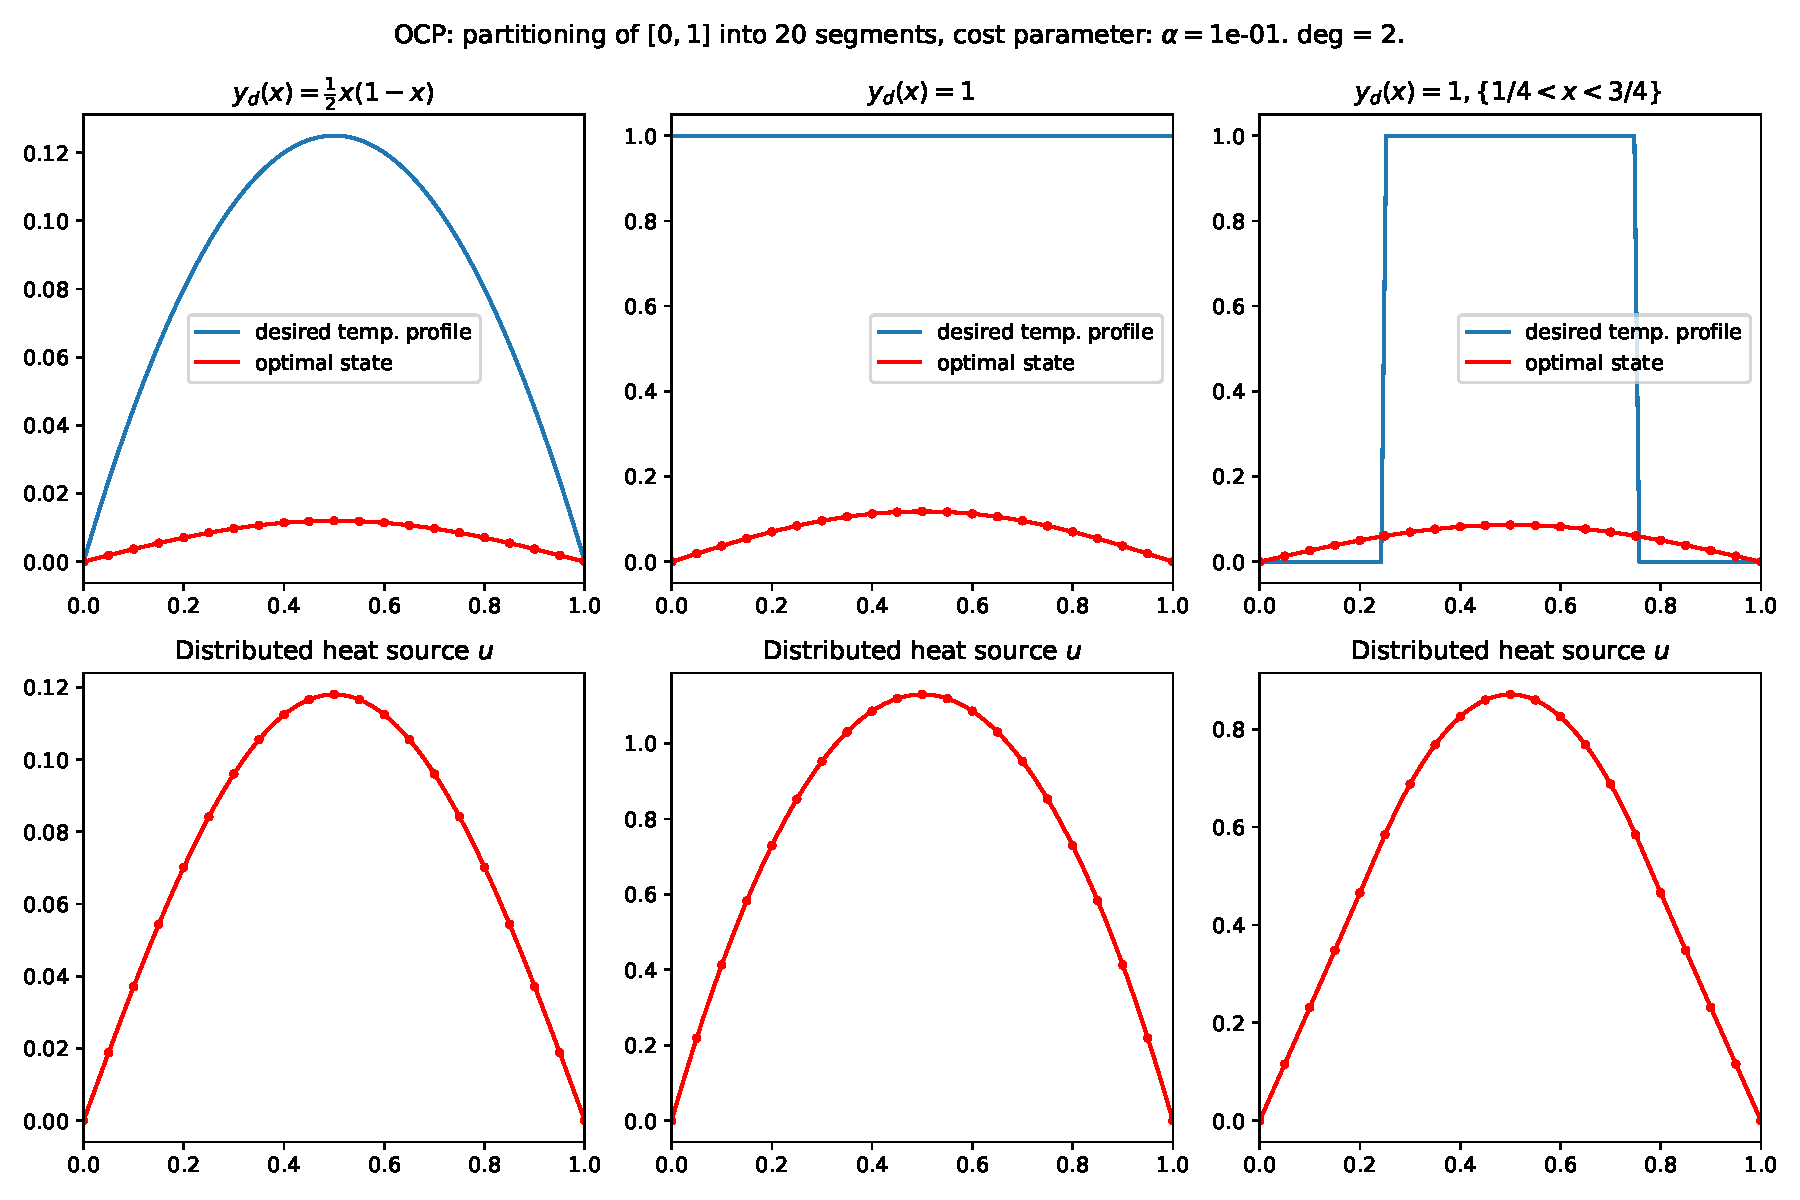
\includegraphics[width=\textwidth]{Images/plots/task2_fig_0.pdf}
  \caption{TODO}
  \label{fig:0}
\end{figure}

\begin{figure}[!h]
  \centering
  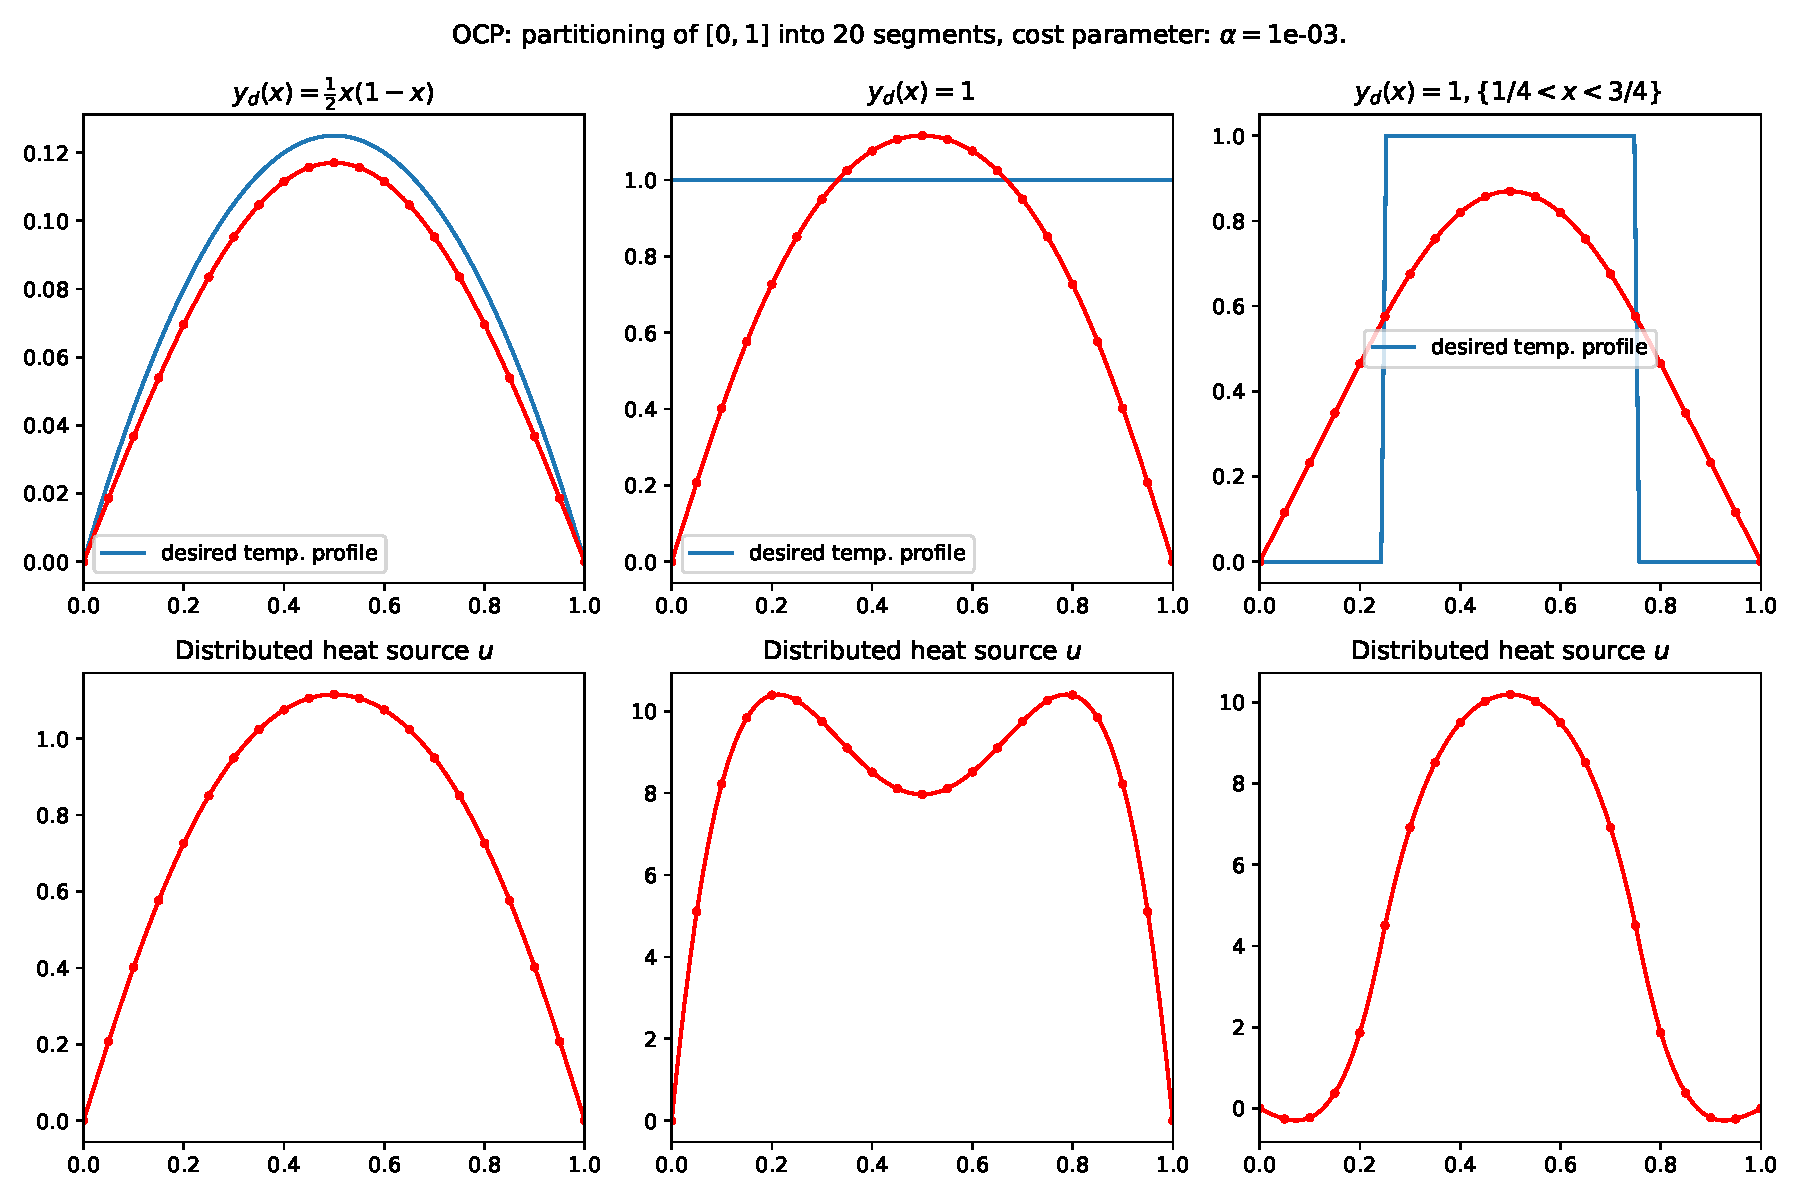
\includegraphics[width=\textwidth]{Images/plots/task2_fig_1.pdf}
  \caption{TODO}
  \label{fig:1}
\end{figure}

\begin{figure}[!h]
  \centering
  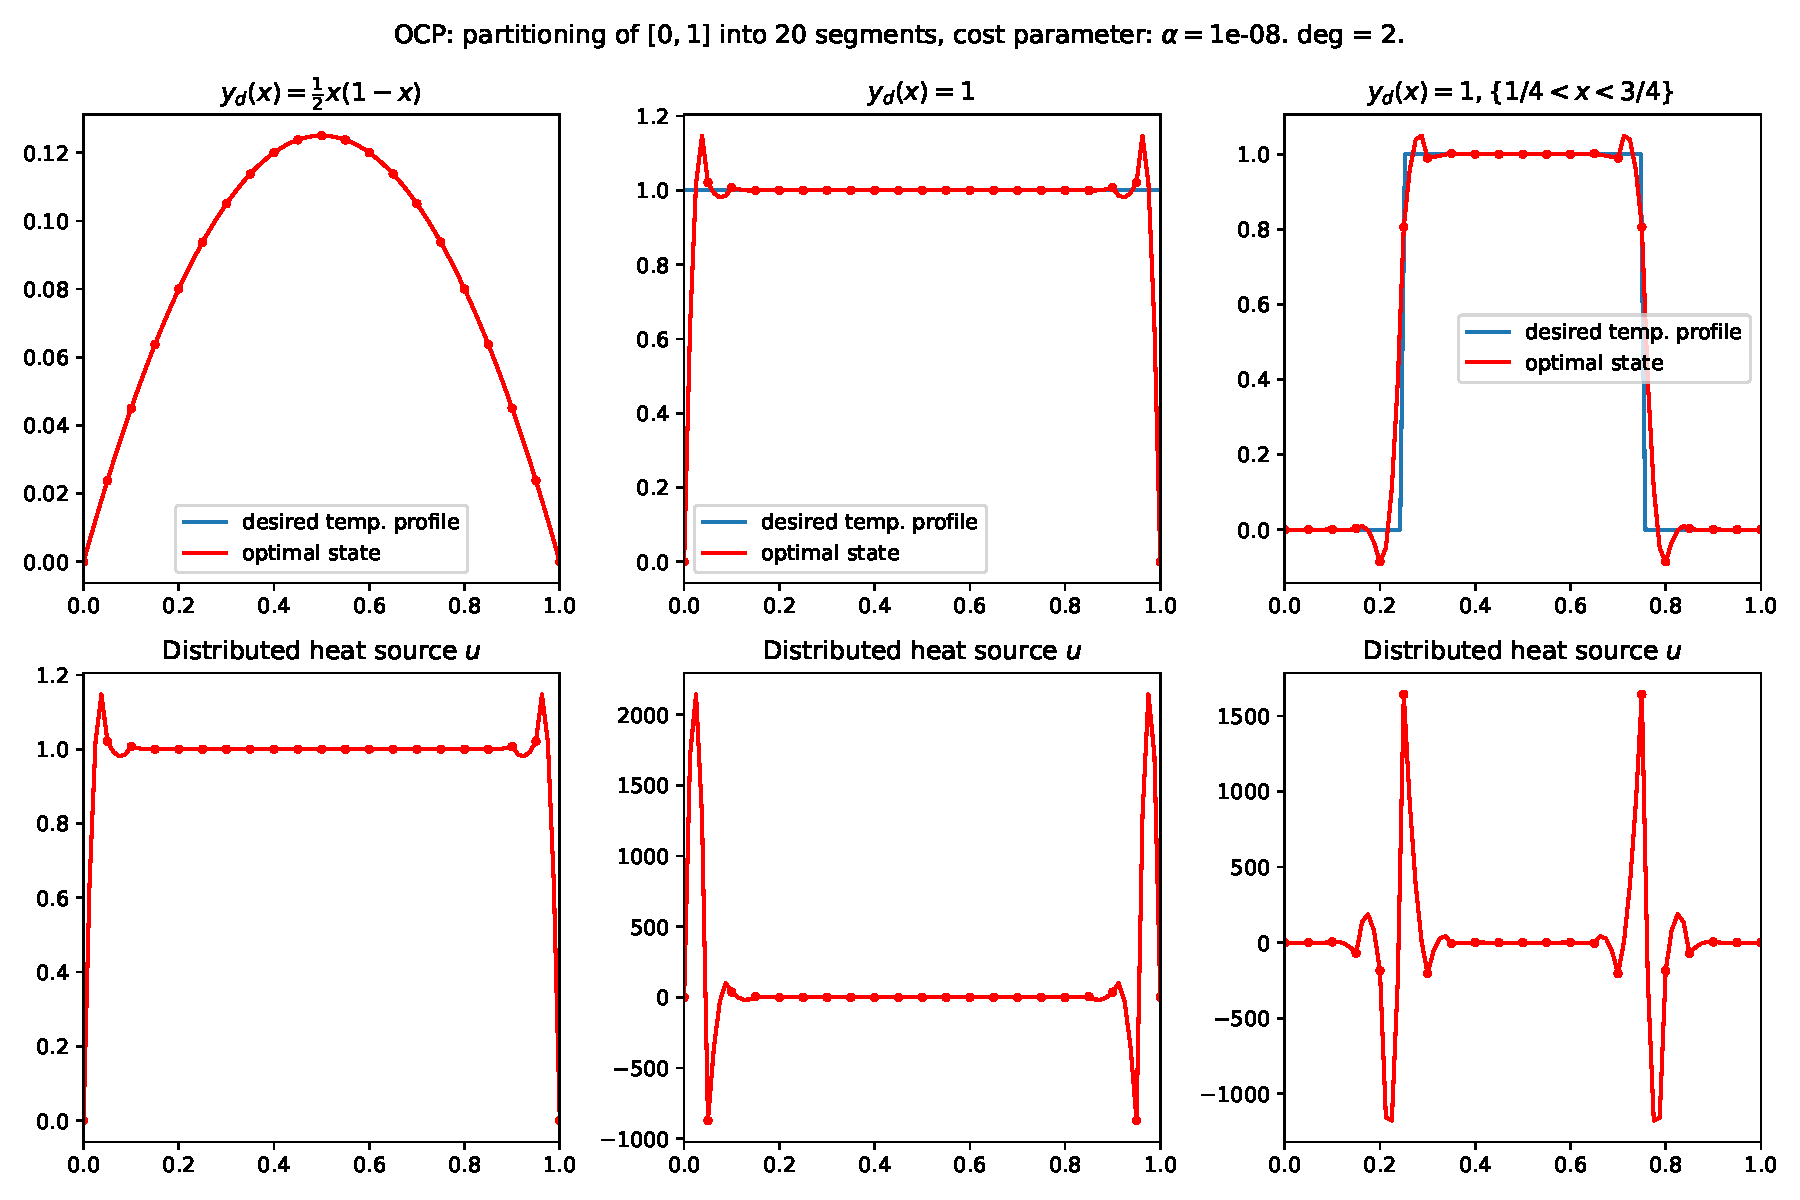
\includegraphics[width=\textwidth]{Images/plots/task2_fig_2.pdf}
  \caption{TODO}
  \label{fig:2}
\end{figure}


